%==============================================================================================
% CONTROL FLOW MANAGER
%==============================================================================================
\section{Control Flow Manager}
\label{sec:cross_domain_linking}
%
Programming errors can cause a module to corrupt its own state.
%
Protection domains created and enforced by the memory map manager cannot prevent such internal memory corruption.
%
Control flow within a system can be affected by internal memory corruption.
%
For example, function pointers (commonly used to implement callbacks) are stored in RAM.
%
Return addresses to function call-sites are stored in the stack.
%
Corruption of these values can cause the processor to execute arbitrary code belonging to the trusted domain.
%
%This violates one of the requirements of using memory map for protection; restricting memory map access to single trusted domain (Refer Section~\ref{subsec:mmap_for_protection}).
%
The Control Flow Manager ensures that control can never flow out of a domain except via calls to functions exported by other domains and via returns to calls from other domains.
%
Conversely, control flow can enter a domain only through an exported function or through the return site of a call that is made to a function exported by some other domain.
%
In addition, the identity of the current domain (that is executing) also needs to be tracked.
%
This information is required by the memory map checker to validate write accesses.
%
%We have implemented a Cross Domain Linking mechanism that is used to transfer control safely from caller to callee domain and vice versa.
%
%A corresponding Cross Domain Return mechanism restores control back to caller domain. 
%
Control flow integrity within a domain is preserved through the safe stack that stores return addresses.
%
%==============================================================================================
% CROSS DOMAIN LINKING
%==============================================================================================
\subsection{Cross Domain Linking}
%
A module loaded in a domain exports a set of functions that can be validly called by modules in other domains.
%
%Cross domain linking enables a module belonging to a domain to call functions in other domain.
%
%Modules in a domain are linked with modules in other domains at load-time.
%
A linker parses the set of functions exported by a domain and writes them to a \textit{jump table} in flash memory.
%
The jump table is similar in design to the processor interrupt vector table.
%
Each entry in the jump table is an instruction to jump to a valid exported function.
%
Each domain has its own jump table that contains all functions that it exports. 
%
Modules are not allowed to directly write to flash memory and therefore the jump table cannot be corrupted.
%
Modules that subscribe to functions exported by a particular domain are re-directed through the jump table of that domain.
%
This is illustrated in Figure~\ref{fig:cross_domain_call}.
%
The jump table mechanism is independent of the process used for dynamic linking i.e. exporting and subscribing to functions.
%
Linking could be done statically or dynamically on the embedded processor~\cite{dunkels06linking}.
%
\begin{figure}[htbp]
   \centering
   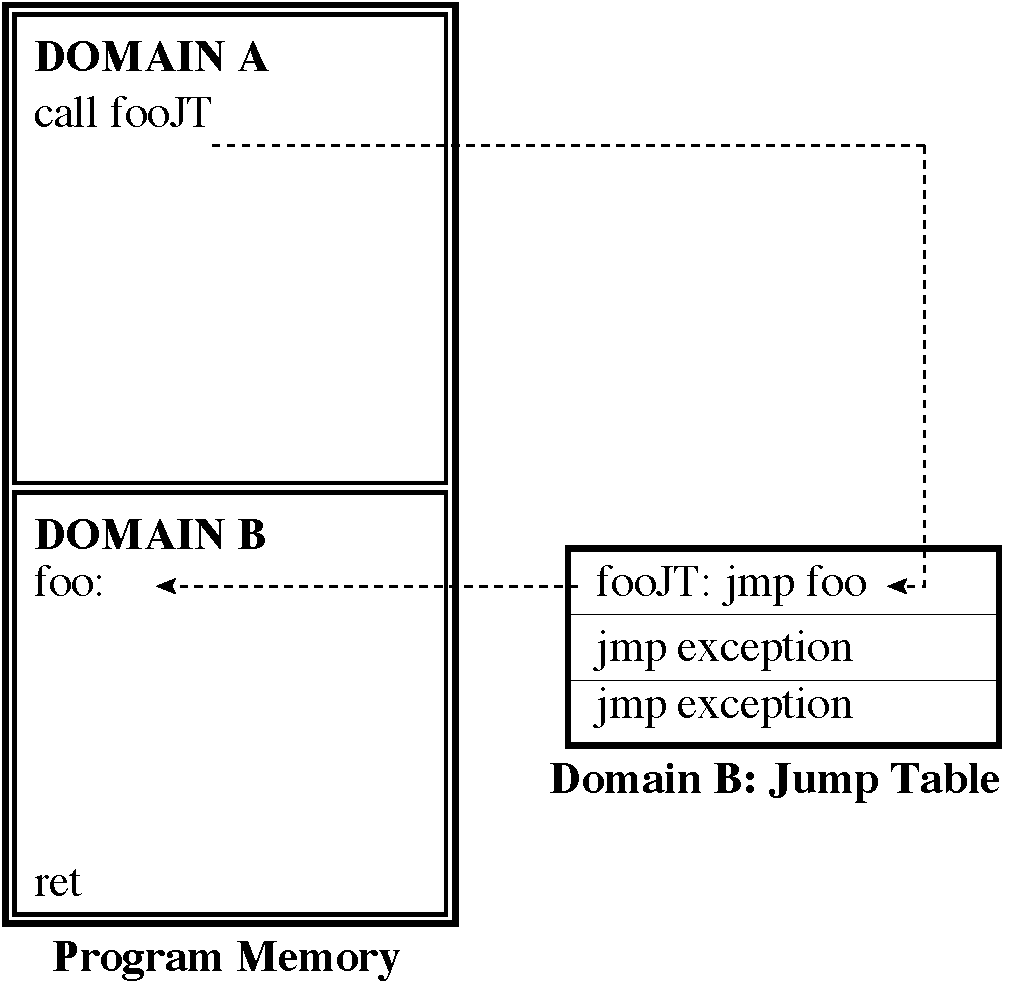
\includegraphics[height=1.75in, keepaspectratio=true]{figures/cross_domain_call.pdf} 
   \caption{Cross Domain Linking}
   \label{fig:cross_domain_call}
\end{figure}
%
%==============================================================================================
% DOMAIN TRACKING
%==============================================================================================
\subsection{Domain Tracking}
%
Domain tracking is performed in hardware by extending the implementation of \texttt{call} and \texttt{return} instructions.
%
Each domain is allocated one complete page of flash memory for storing its jump table.
%
In AVR architecture this imposes a limit of 128 functions that can be exported by every domain.
%
This limit can be easily extended by allocating more space to the jump table.
%
%The maximum number of exported functions by any SOS module is 12.
%
Empty entries in the jump table are filled with a jump instruction to an exception routine.
%
Jump table pages of all domains are co-located and stored at fixed location in flash memory.
%

This organization simplifies the algorithm for verifying the target address of a call.
%
A valid target address has to reside in the jump table.
%
This is checked by a simple compare operation to the base address of the jump table.
%
The check against the upper bound of jump table is deferred.
%
%and stack bound need to be stored in a stack.


The identity of the called domain is also easily determined.
%
Jump tables of all domains are organized linearly, starting from the domain 0 jump table located at the base address.
%
The identifier of the target domain can be easily determined by first computing the address offset from the base address of the jump table and dividing it by the size of the jump table.
%
If the target domain identifier exceeds the maximum number of domains in the system, then it indicates that the target address is greater than the upper bound of the jump table, and an exception is generated.
%
Finally, a call is made into the jump table that is redirected to the actual entry point in the target domain.
%

The current domain identifier needs to be pushed to a stack, because cross domain calls can be chained: domain A calls domain B which in turn calls domain C.
%
During cross domain return, the previous domain identifier is restored and the control is transferred back to the caller's domain.
%
The cross domain state machine handles the push and pop operations transparently to the application programs.
%
%All function calls made across domains pass through a \textit{jump table} setup in the program memory.
%
%Four operations are performed by the cross domain call stub.
%
%First, it verifies target address of the call.
%
%A valid target address should match the address of any exported function.
%
%Second, it determines the identity of callee domain and stores it.
%
%Third, it saves the return address of caller domain.
%
%Fourth, it sets up a stack bound.
%
%Stack bound is required for stack protection (Section~\ref{subsec:stackguard}).
%
%Cross domain call stub resides within the single trusted domain.
%
%Design of calling mechanism tries to optimize performance overhead of these operations.
%
%
%==============================================================================================
% STACK PROTECTION
%==============================================================================================
\subsection{Run-Time Stack Protection}
\label{subsec:stackguard}
%
Embedded micro-controllers have a single execution stack that is shared by the entire system.
%
In most architectures, the stack is initialized at the end of address space and grows down towards the start of address space.
%
The run-time stack is used for many purposes.
%
First, it is used to record the return addresses of function calls.
%
Second, it is used to set up data frames for storing local variables or function arguments that cannot be accommodated in registers.
%
Third, it is also used to store arguments for variadic functions.
%
Stack corruption is a serious problem.
%
Our protection model prevents corruption of the stack belonging to one domain by any module belonging to a different domain.
%
During a cross domain call  the processor copies the current stack pointer into a \texttt{stack\_bound} register. 
%
The previous stack bound is saved.
%a stack bound is setup before control is transferred from one domain to another.
%
The memory map checker compares the write address to the current stack bound and signals an exception if the address exceeds the stack bound.
%disallows writes to memory addresses greater than current stack bound.
%
%As shown in figure~\ref{fig:checker}, stack access checker is invoked if the write address points to stack.
%
%Stack access checker 
%
Therefore, modules belonging to a domain cannot corrupt the stack belonging to another domain.
%
%==============================================================================================
% SAFE STACK
%==============================================================================================
\subsection{Safe Stack}
%
A module can call any local function within its domain.
%
The return address of function calls are stored in stack and are protected from corruption from modules in other domains.
%
However, a programming error can cause a module to corrupt its own stack.
%
This cannot be prevented by protection domains.
%
Therefore, we store all return addresses in a separate stack that resides in a different protection domain.
%
We call this a safe stack.
%
%Entry (and exit point) of every local function in a domain is re-written to invoke a stub routine that pushes (and pops) return addresses into the Safe Stack.
%
%Safe Stack pointer is maintained as a global variable that is read (and written) before (and after) a sequence of push/pop operations. 
%
%Safe Stack is used to overwrite return address values in run-time stack.
%
%We do not modify run-time stack in any manner as it would corrupt data frames setup by functions for storing local data and function arguments.
%
A safe stack can be setup only by the software in the trusted domain by writing to the \texttt{safe\_stack\_ptr}.
%
The safe stack can be setup anywhere in data memory as long as it is protected from accidental writes and overflow.
%
We usually setup Safe Stack at the end of all global data in the system and make it grow upwards.
%
Run-Time stack and Safe Stack approach one another.
%
%Binary rewriter introduces the stubs to push and pop into Safe Stack.
%
%Therefore, all return addresses are checked.
%
%Domains occupy contiguous portions in program memory. 
%
%When the domain is loaded into a system, the Control flow manager records its start and end addresses.
%
%Return addresses are checked to ensure that they lie within bounds of the current domain; else an exception is raised.
%
%Similarly, all computed call addresses are also subject to an identical bounds check.
%
%Calls to static addresses are verified at load time.
%
%All checks are introduced through a binary rewriter.













